%% LyX 2.3.2 created this file.  For more info, see http://www.lyx.org/.
%% Do not edit unless you really know what you are doing.
\documentclass{article}
\usepackage{courier}
\usepackage[T1]{fontenc}
\usepackage[utf8]{inputenc}
\usepackage[spanish]{babel}
\usepackage{subfiles}
\usepackage{geometry}
\usepackage{amsmath}
\usepackage{amsfonts}
\geometry{verbose,tmargin=2cm,bmargin=2cm,lmargin=1.5cm,rmargin=1.5cm}
\usepackage{multicol}
% \usepackage{graphicx}
\usepackage{array}
\usepackage{framed}
\usepackage{listings}
\usepackage{color}
\usepackage{enumitem}
\usepackage{xcolor}
\usepackage{colortbl}
\usepackage{wrapfig}
\usepackage{sectsty} % change section size
\setlength{\parskip}{1em}
\usepackage{float}
\usepackage{hyperref}
\usepackage[backend=biber,style=numeric,
            sorting=nyt]{biblatex} % Complete reimplementation of bibliographic facilities
%\addbibresource{bibliography.bib}
\usepackage{amsthm}



\newtheorem{definition}{Definición}[section]
\newtheorem{theorem}{Teorema}[section]
\newtheorem{remark}{Observación}[section]
\newtheorem{corollary}{Corolario}[theorem]
\newtheorem{lemma}{Lema}[theorem]

\makeatletter


\sectionfont{\fontsize{12}{16}\selectfont}
\subsectionfont{\fontsize{10}{14}\selectfont}

\providecommand{\tabularnewline}{\\}

\definecolor{mygreen}{rgb}{0,0.6,0}
\definecolor{mygray}{rgb}{0.5,0.5,0.5}
\definecolor{mymauve}{rgb}{0.58,0,0.82}

\usepackage{listings}
\definecolor{background}{rgb}{0.97,0.97,0.97}
\definecolor{mygreen}{rgb}{0.1,0.6,0.1}
\definecolor{mygray}{rgb}{0.5,0.5,0.5}
\definecolor{mymauve}{rgb}{0.58,0,0.82}

\renewcommand{\lstlistingname}{Código}
\renewcommand{\lstlistlistingname}{Índice de códigos}
\lstset{ 
  title=Fichero \lstname,          % show the filename of files included with \lstinputlisting; also try caption instead of title
  caption=Fichero \lstname,
  captionpos=t,                    % sets the caption-position (b/t)
  frame=shadowbox,                       % adds a frame around the code
  rulecolor=\color{black},         % if not set, the frame-color may be changed on line-breaks within not-black text (e.g. comments (green here))
  numbers=left,                    % where to put the line-numbers; possible values are (none, left, right)
  numbersep=10pt,                  % how far the line-numbers are from the code
  stepnumber=0,                    % the step between two line-numbers. If it's 1, each line will be numbered
  backgroundcolor=\color{background},
  numberstyle=\small\color{mygray},% the style that is used for the line-numbers
  basicstyle=\footnotesize\selectfont\ttfamily, % the size/type of the fonts that are used for the code
  keywordstyle=\color{blue},       % keyword style
  commentstyle=\color{mygreen},    % comment style
  stringstyle=\color{mymauve},     % string literal style
  breakatwhitespace=false,         % sets if automatic breaks should only happen at whitespace
  breaklines=true,                 % sets automatic line breaking
  keepspaces=true,                 % keeps spaces in text, useful for keeping indentation of code (possibly needs columns=flexible)
  showstringspaces=false,          % underline spaces within strings only
  showspaces=false,                % show spaces everywhere adding particular underscores; it overrides 'showstringspaces'
  showtabs=false,                  % show tabs within strings adding particular underscores
  tabsize=2,                     % sets default tabsize to 2 spaces
  language=SQL,                    % the language of the code
  morekeywords={REFERENCES, NVL, ROUND},            % if you want to add more keywords to the set
  deletekeywords={},            % if you want to delete keywords from the given language
  %escapeinside={--}{\^^M},          % if you want to add LaTeX within your code
  extendedchars=true,              % lets you use non-ASCII characters; for 8-bits encodings only, does not work with UTF-8
  literate=
  {á}{{\'a}}1 {é}{{\'e}}1 {í}{{\'i}}1 {ó}{{\'o}}1 {ú}{{\'u}}1
  {Á}{{\'A}}1 {É}{{\'E}}1 {Í}{{\'I}}1 {Ó}{{\'O}}1 {Ú}{{\'U}}1
  {à}{{\`a}}1 {è}{{\`e}}1 {ì}{{\`i}}1 {ò}{{\`o}}1 {ù}{{\`u}}1
  {À}{{\`A}}1 {È}{{\'E}}1 {Ì}{{\`I}}1 {Ò}{{\`O}}1 {Ù}{{\`U}}1
  {ä}{{\"a}}1 {ë}{{\"e}}1 {ï}{{\"i}}1 {ö}{{\"o}}1 {ü}{{\"u}}1
  {Ä}{{\"A}}1 {Ë}{{\"E}}1 {Ï}{{\"I}}1 {Ö}{{\"O}}1 {Ü}{{\"U}}1
  {â}{{\^a}}1 {ê}{{\^e}}1 {î}{{\^i}}1 {ô}{{\^o}}1 {û}{{\^u}}1
  {Â}{{\^A}}1 {Ê}{{\^E}}1 {Î}{{\^I}}1 {Ô}{{\^O}}1 {Û}{{\^U}}1
  {œ}{{\oe}}1 {Œ}{{\OE}}1 {æ}{{\ae}}1 {Æ}{{\AE}}1 {ß}{{\ss}}1
  {ű}{{\H{u}}}1 {Ű}{{\H{U}}}1 {ő}{{\H{o}}}1 {Ő}{{\H{O}}}1
  {ç}{{\c c}}1 {Ç}{{\c C}}1 {ø}{{\o}}1 {å}{{\r a}}1 {Å}{{\r A}}1
  {€}{{\euro}}1 {£}{{\pounds}}1 {«}{{\guillemotleft}}1
  {»}{{\guillemotright}}1 {ñ}{{\~n}}1 {Ñ}{{\~N}}1 {¿}{{?`}}1
}




\makeatother
\begin{document}
\begin{center}
  \Large\textbf{Métodos Numéricos de las Ecuaciones Diferenciales}\\
  \line(1,0){450}
\end{center}

\section{Resolución numérica de problemas de valor inicial para EDO}

\begin{definition}
    Llamamos problema de valor inicial a una EDO junto a una condición inicial:
\begin{equation} \label{eqn:pvi}
\begin{cases}
    y'(t)=f(t.y(t)) \\
    y(a) = y_0 \\
    t\in[a,b]
\end{cases}
\end{equation}
\end{definition}

\begin{remark}Los problemas que trataremos serán de orden 1 siempre, en otro caso los transformaremos en problemas de mayor dimensión \end{remark}
\begin{remark}Sería más correcto escribir $\vec y$, pues pueden ser funciones vectoriales, pero por facilidad lo omitiré. \end{remark}

    Los métodos que veremos calcularán soluciones del PVI \ref{eqn:pvi} como una lista de pares $[(t_0,w_0), \dots, (t_n,w_n)]$, dónde los $t_i$ son reales de forma que $a=t_0<t_1<\dots < t_n\geq b$ y los $w_i$ son vectores que aproximan a la solución real en los $t_i$: $y(t_i)\approx w_i,\forall i=0,\dots, n$.

\begin{remark} Por supuesto, al implementarlo usaremos números máquina, no reales matemáticos.  \end{remark}
\begin{remark} Si queremos obtener una aproximación en cualquier punto del intervalo tenemos que usar una interpolación adecuada. \end{remark}

\section{Métodos de paso fijo}

\begin{definition}  Un método es de paso fijo si la solución que genera cumple $t_i-t_{i-1}=h,\forall i=1,\dots n$ para cierto $h>0$ constante. \end{definition}

En este caso se tendrá $n=\lceil \frac{b-a}{2} \rceil$, y supondré este valor mientras trate con métodos de paso fijo.

\subsection{Método de Euler}
\begin{definition} 
    El método de Euler de paso fijo genera, dado el problema \ref{eqn:pvi} y un paso $h>0$:

\begin{equation} \label{eqn:eulersol}
\begin{cases}
    w_0=y_0 \\
    w_{i+1}=w_i + h\cdot f(t_i, w_i), \forall i=0,\dots, n-1
\end{cases}
\end{equation}

Siendo $t_i =t_0+i\cdot h,\forall i=0,\dots, n$.
\end{definition}

\subsubsection{Estimación del error con el método de Euler}

\begin{theorem}[Convergencia del método de Euler]
    Sea $f:D\subset \mathbb{R}^2\rightarrow \mathbb{R}$ con $D$ abierto, e $Y(t)$ una solución de $(1)$ con $(t,Y(t))\in D,\forall t\in[a,b]$. Sea también la solución \ref{eqn:eulersol} para cierto $h$ fijo. Si se cumple
    \begin{enumerate}[label=(\alph*)]
        \item f Lipschitziana respecto de la segunda variable en $D$, con constante de Lipschitz $K$.
        \item $Y''$ existe en todo $[a,b]$ y está acotada por una constante $C\geq 0$.
        \item $(t_i,w_i)\in D,\forall i=0,\dots,n$.
    \end{enumerate}
    entonces $$\max_{0\leq i \leq n}|Y(t_i)-w_i| \leq e^{(b-a)K}\cdot |Y(a)-w_0| + \frac{e^{(b-a)K}-1}{2K}ch$$

\end{theorem}
\begin{proof}
% TODO
\end{proof}

\begin{theorem}[Convergencia del método de Euler con error de redondeo]
    Sea $f:D\subset \mathbb{R}^2\rightarrow \mathbb{R}$ con $D$ abierto, e $Y(t)$ una solución de $(1)$ con $(t,Y(t))\in D,\forall t\in[a,b]$.

    Fijado $h>0$, sea la solución numérica

\begin{equation}
\begin{cases}
    w_0=y_0 \\
    w_{i+1}=w_i + h\cdot f(t_i, w_i) + \delta_i
\end{cases}
\end{equation}

con $\delta_i<\delta,\forall i=0,\dots,n$.

    Si se cumple
    \begin{enumerate}[label=(\alph*)]
        \item f Lipschitziana respecto de la segunda variable en $D$, con constante de Lipschitz $K$.
        \item $Y''$ existe en todo $[a,b]$ y está acotada por una constante $C\geq 0$.
        \item $(t_i,w_i)\in D,\forall i=0,\dots,n$.
    \end{enumerate}
    entonces $$\max_{0\leq i \leq n}|Y(t_i)-w_i| \leq e^{(b-a)K}\cdot |Y(a)-w_0| + \frac{e^{(b-a)K}-1}{K}\left(\frac{1}{2}ch+\frac{\delta}{h}\right)$$

\end{theorem}

Se puede estimar el error de otra forma bajo ciertas condiciones, que nos será muy útil para estimar numéricamente el error e incluse obtener soluciones mejores a partir del método de Euler.

\begin{theorem}
    Dado el PVI \ref{eqn:pvi} y la solución \ref{eqn:eulersol}, si la solución $Y(t)$ real es de clase $C^3$ y $\frac{\partial f}{\partial y},\frac{\partial^2f}{\partial y^2}$ constantes, entonces
    \begin{equation}
    Y(t_i)-w_i=h\cdot D(t_i)+\theta(h^2),\forall t\in[t_0,b]
    \end{equation}
    dónde $D$ es solución del siguiente PVI:
\begin{equation}
\begin{cases}
    d'(t)=g(t)d(t) + \frac{1}{2} Y''(t), g(t)=\frac{\partial f(t,y)}{\partial y}(t,Y(t)) \\
    d(a) = 0 \\
    t\in[a,b]
\end{cases}
\end{equation}
\end{theorem}
\begin{proof}
Puede encontrarse en el libro de Atkinson, pero no entra.
\end{proof}

\begin{theorem}
    En condiciones similares a las del teorema anterior, tomando $(t_i^h,w_i^h)$ y $(t_i^{h/2},w_i^{h/2})$ soluciones obtenidas con el método de Euler con pasos $h$ y $\frac{h}{2}$ respectivamente:
    \begin{enumerate}[label=(\alph*)]
        \item $Y(t_i^h)-w_{2i}^{h/2} = (w_{2i}^{h/2}-w_i^h) + \theta(h^2)$.
        \item $w_i := 2\cdot w_{2i}^{h/2}-w_i^h$ es una aproximación de $Y(t)$ de orden $\theta(h^2)$.
    \end{enumerate}
\end{theorem}

\begin{proof}
    Aplicando el teorema anterior obtenemos:
    $$
    Y(t_i^h)-w_i^h=h\cdot D(t_i^h)+\theta(h^2),\forall t\in[t_0,b]
    $$
    $$
    Y(t_{2i}^{h/2})-w_{2i}^{h/2}=h\cdot D(t_{2i}^{h/2})+\theta(h^2),\forall t\in[t_0,b]
    $$
    Basta observar que $t_i^h = t_{2i}^{h/2}$ y restar la primera ecuación a la segunda multiplicada por 2. Despejando se obtiene tanto (a) como (b).

\end{proof}

\subsection{Estimación general del error}

Como hemos visto, a partir de conocer el error cometido en cada paso hemos logrado estimar globalmente el error de la solución generada por el método de Euler. La idea es hacer esto de manera general, pero de momento nos conformamos con formalizar la idea de error local.

\begin{definition}
Dado un método de diferencias
\begin{equation} \label{eqn:diffmet}
\begin{cases}
    w_0=\alpha \\
    w_{i+1}=w_i + h\cdot \phi(t_i, w_i), \forall i=0,\dots, n-1
\end{cases}
\end{equation}
    que devuelva una solución de \ref{eqn:pvi} con solución real $Y$, se define su \textbf{error local de truncamiento (e.l.t.)} como
    $$
    T_{i+1}(h) = \frac{Y(t_{i+1})-Y(t_i)-h\phi(t_i,Y(t_i))}{h}
    = \frac{Y(t_{i+1})-Y(t_i)}{h} -h\phi(t_i,Y(t_i))
    $$
\end{definition}


En el caso concreto del método de Euler se tiene:
    $$
    T_{i+1}(h)
    = \frac{Y(t_{i+1})-Y(t_i)}{h} -h\cdot f(t_i,Y(t_i))= \frac{h}{2} Y''(\xi_i),
    \xi_i\in[t_i,t_{i+1}], \forall i=0,\dots, n-1
    $$

    y si $|Y''(t)|\leq C,\forall t\in[a,b]$ entonces
    $$
    |T_{i+1}(h)|\leq \frac{C}{2} \cdot h
    $$
    que es $\theta(h)$.

Lo que nos interesa es que este error decrezca lo más rápido posible con h, es decir, que sea $\theta(h^p)$ con $p$ lo más grande posible. En esta búsqueda llegamos al siguiente método, el de Taylor.

\subsection{Método de Taylor}
 
De aquí en adelante asumiré el PVI general del principio, y cualquier método que considere intentará aproximar una solución suya.

\begin{definition}
Se define el método de Taylor de orden p como:
\begin{equation} \label{eqn:diffmet}
\begin{cases}
    w_0=\alpha \\
    w_{i+1}=w_i + h\cdot T^{(p)}(t_i, w_i), \forall i=0,\dots, n-1
\end{cases}
\end{equation}

    dónde $T^{(p)}(t_i,w_i)=\sum_{i=0}^{p-1} \frac{h^i}{(i+1)!}f^{(i)}(t_i,w_i)$, y $f^{(i)}(t_i,w_i)$ viene dado po $Y^{(i+1)}(t)=(f(t,Y(t)))^{(i)}$.
\end{definition}

Unas pocas cuentas son suficientes para darse cuenta de que calcular estas derivadas de manera genérica es realmente costoso, y normalmente se suelen hace las cuentas de manera \textit{adhoc} para un problema concreto.

El siguiente teorema era de esperar:

\begin{theorem}
    Si Y es de clase $C^{(p+1)}([a,b])$, el e.l.t. del método de Taylor de orden p es $\theta(h^p)$.
\end{theorem}
\begin{proof}
En estas condiciones el e.l.t. no es más que el resto de Lagrange:

$$
    T_{i+1}(h)=\frac{h^p}{(p+1)!} f^{(p)}(\xi_i,Y(\xi_i)),\xi_i\in [t_i,t_{i+1}]\subset[a,b]
$$
    Por ser $f(t,Y(t))$ contínua en compacto está acotada en $[a,b]$, y eso es por lo tanto $\theta(h^p)$.
\end{proof}

%TODO esto solo para una dimensión?

A pesar de este gran resultado respecto al error, la dificultad para aplicarlo de manera genérica y los problemas que conlleva la derivación numérica no lo hace muy práctico. Buscamos entonces métodos que no necesiten estas derivadas y que tengan órdenes similares.

\subsection{Métodos de Runge-Kutta}

Comenzamos buscando métodos de orden 2, para lo cual queremos aproximar $T^{(2)}(t,y)=f(t,y)+\frac{h}{2} f'(t,y)$ con un error de orden $\theta(h^2)$. Una idea feliz es considerar una aproximación de la forma $a_1f(t+\alpha_1, y+\beta_1)$. Aproximando esto último por Taylor tenemos:

$$
a_1f(t+\alpha_1, y+\beta_1)=a_1\left(
f(t,y)+
\frac{\partial f}{\partial t}(t,y)\cdot \alpha_1+
\frac{\partial f}{\partial y}(t,y)\cdot \beta_1+
\frac{\partial^2 f}{\partial t^2}(\xi,\mu)\cdot \frac{\alpha_1^2}{2}+
\frac{\partial^2 f}{\partial t \partial y}(\xi,\mu)\cdot \alpha_1\beta_1+
\frac{\partial^2 f}{\partial y^2}(\xi,\mu)\cdot \frac{\beta_1^2}{2}
\right)
$$

Nótese que suponemos suficiente regularidad en f para que las parciales cruzadas sean iguales. Haciendo $a_1=1,\alpha_1=\frac{h}{2}, \beta_1=\frac{h}{2} f(t,y)$ la igualdad anterior se traduce en:

$$
f(t+\frac{h}{2}, y+\beta_1)=
f(t,y)+
\frac{\partial f}{\partial t}(t,y)\cdot \frac{h}{2}+
\frac{\partial f}{\partial y}(t,y)\cdot \frac{h}{2} f(t,y)+
\frac{\partial^2 f}{\partial t^2}(\xi,\mu)\cdot \frac{h^2}{8}+
\frac{\partial^2 f}{\partial t \partial y}(\xi,\mu)\cdot \frac{h^2}{4}f(t,y)+
\frac{\partial^2 f}{\partial y^2}(\xi,\mu)\cdot \frac{h^2}{8}f(t,y)
$$

$$
=T^{(2)}(t,y)+
h^2 \left(
\frac{\partial^2 f}{\partial t^2}(\xi,\mu)\cdot \frac{1}{8}+
\frac{\partial^2 f}{\partial t \partial y}(\xi,\mu)\cdot \frac{1}{4}f(t,y)+
\frac{\partial^2 f}{\partial y^2}(\xi,\mu)\cdot \frac{1}{8}f(t,y)
\right)
$$

De nuevo bajo buenas condiciones de $f$ lo que hay entre paréntesis está acotado, y al multiplicar por $h^2$ tenemos el orden de error buscado. Esto nos da nuestro primer método de Runge-Kutta:

\begin{definition}
    El método del Punto Medio viene dado por
\begin{equation} \label{eqn:diffmet}
\begin{cases}
    w_0=\alpha \\
    w_{i+1}=w_i + h\cdot f(t+\frac{h}{2}, y+\frac{h}{2}f(t,y)) , \forall i=0,\dots, n-1
\end{cases}
\end{equation}
\end{definition}

\begin{remark}
    En este método no necesitamos solo necesitamos la función $f$, pero necesitamos dos evaluaciones en cada paso, que puede ser costoso.
\end{remark}

\begin{remark}
    Al ser $ f(t+\frac{h}{2}, y+\beta_1)=T^{(2)}(t,y)+\theta(h^2) $, el e.l.t. será:
    $$
    T_{i+1}(h)= \left(\frac{}{h} - T^{(2)}(t_i, y(t_i))\right) - \theta(h^2)
    =\theta(h^2)+ \theta(h^2)
    =\theta(h^2)
    $$
\end{remark}

%TODO reflexión para orden 3

Es fácil ver que si queremos más precisión tenemos que utilizar más evaluaciones de $f$. Una pregunta interesante es el número mínimos de evaluaciones en cada paso para conseguir una aproximación de cierto orden. La siguiente tabla relaciona ambos conceptos:

\begin{table}[H]
\centering
\begin{tabular}{|l||l|l|l|l|}
    \hline
Evaluaciones & $1\leq p \leq 4$ & $5\leq p\leq 7$ & $8\leq p\leq 9$  & $10\leq p$ \\
    \hline
Mejor e.l.t. & $\theta(h^p)$ & $\theta(h^{p-1})$ & $\theta(h^{p-2})$ & $\theta(h^{p-3})$ \\
    \hline
\end{tabular}
\caption{Tabla de Butcher de evaluaciones y órdenes del e.l.t.}
\end{table}

Muchas veces utilizamos el número de evaluaciones de la función $f$ como medida de complejidad, pues puede se muy costosa.

Tenemos también dos formas de mejora la precisión de la solución numérica: reducir el paso y usar un método de orden mayor. Veamos la comparación de estas dos formas con los métodos de Runge-Kutta vistos hasta el momento, fijando el número de evaluaciones a $40$ y suponiendo un intervalo con $b-a=1$:

\begin{table}[H]
\centering
\begin{tabular}{|l|l|l|}
    \hline
Método           & Paso  & Precisión aproximada \\
    \hline
    \hline
RK4              & 0.1   & $10^{-4}$ \\
    \hline
Euler Modificado & 0.05  & $2.5\cdot 10^{-3}$ \\
    \hline
Euler            & 0.025 & $2.5\cdot 10^{-2}$ \\
    \hline
\end{tabular}
\end{table}

En general obtenemos mejores resultados aumentando el orden del método.


\section{Métodos de paso adaptativo}

\section{Rigidez}

La rigidez es un fenómeno que asociamos a un problema de valor inicial.
Más que una característica matemática,
que podría ser definida de forma precisa,
es un conjunto de complicaciones que surgen
en la resolución de ciertos problemas.

\subsection{Un primer problema rígido}

Consideremos el problema de valor inicial
%
\begin{equation}\label{prb:rigid1}
    \begin{cases}
        y'(t) = 5\nume^{5t}(y-t)^2 + 1 \\
        y(0)
    \end{cases}
    \qq{para $t$ en $[0,1]$ o $[0,8]$}
\end{equation}
%
cuya solución analítica es $y(t) = t - \nume^{-5t}$.
Si intentamos resolverlo con el método de RK4
podemos construir la tabla \cref{tab:rigid-problem-rk4-step-error-comparison}.
Observamos un fenómeno extraño.
Si el paso es menor que $0.2419$
el método obtiene unas cotas de error razonables
que se van reduciendo conforme disminuímos el tamaño del paso.
Sin embargo, si el paso es mayor o igual que $0.2419$,
el error del método se dispara.

\begin{table}[h]
    \centering
    \begin{tabular}{lll}
        \textbf{Tam. paso} & \textbf{Error Abs.} & \textbf{Error Rel.} \\
        \hline \\
        0.2001 & 0.0192308 & 0.00123008 \\
        0.2101 & 0.0463702 & 0.00266692 \\
        0.2201 & 0.0914377 & 0.00529422 \\
        0.2301 & 0.163178  & 0.0101477 \\
        0.2411 & 0.287569  & 0.0215778 \\
        0.2413 & 0.290396  & 0.0220027 \\
        0.2415 & 0.293245  & 0.0224769 \\
        0.2417 & 0.296118  & 0.0230281 \\
        0.2419 & inf       & inf \\
        0.2421 & inf       & inf \\
        0.2423 & inf       & inf
    \end{tabular}
    \caption{Error del método de RK4 para resolver el \cref{prb:rigid1}}
    \label{tab:rigid-problem-rk4-step-error-comparison}
\end{table}

Cuando integramos una ecuación diferencial cuyas derivadas tenemos acotadas,
la intuición\footnote{
    Justificada por las fórmulas de error que hemos obtenido,
    ya que una aproximación del error es $Cy^{(p)}(\xi)h^p$.
}
nos dice que el tamaño del paso
podría ser grande en zonas donde la variación de la curva es pequeña
y debería ser más pequeño en intervalos donde la variación es grande.
También asumimos que podemos controlar el error
eligiendo un tamaño de paso adecuado o
obtener una aproximación del mismo
comparando una solución con otra donde hemos reducido el tamaño del paso.
Sin embargo, en el problema anterior vemos que el error,
si el paso no es más pequeño que un umbral\footnote{
    Podemos probar con otros métodos de paso fijo.
    Veremos que el umbral cambia en función del método.
},
se dispara.
Y por tanto la solución que estamos calculando
no converge paulatinamente hasta ese valor.

\subsection{Definición}

La característica que hemos visto no es atribuíble a la solución
$y(t) = t - \nume^{-5t}$,
puesto que podemos cambiar el problema para que siga teniendo la misma solución
y no se dispare el error.
Por tanto, la rigidez es una característica de un problema de valor inicial,
y no de una solución a ese problema.

Aparte del fenómeno anterior,
hay otros que habitualmente se atribuyen a los problemas que llamamos rígidos.
Enumeramos tres.
%
\begin{enumerate}
    \item Si el paso no está por debajo de un umbral,
    el error se dispara.
    \item Si utilizamos un método de paso adaptativo para resolver el problema,
    el método acaba porque sobreestima el error y determina que
    el paso que necesitaría utilizar sería menor que el mínimo permitido.
    Es un fenómeno que también se da en el problema anterior,
    pero si comparamos con la solución analítica vemos que en realidad
    el error del método cumple la tolerancia pedida.
    \item Si utilizamos un método de paso fijo tradicional,
    obtenemos una solución que oscila alrededor de la solución analítica.
    Por tanto, aunque la aproxime bien lo hace con un comportamiento diferente.
\end{enumerate}

Querríamos dar una definición precisa de problema rígido
basada en estos fenómenos.
Sin embargo, para cualquiera de ellos, podemos encontrar problemas
que nuestra definición tiene que considerar rígidos porque
presentan el resto de los fenómenos
pero que excluirían ese.
Lo que sí podemos es reconocer características que son comunes
a los problemas que presenten estos fenómenos.

Por ejemplo,
un sistema lineal de coeficientes constantes podría definirse como rígido
cuando todos sus valores propios, $\lambda_1,\ldots,\lambda_n$,
tienen parte real negativa y el coeficiente
%
\begin{equation*}
    \frac{\abs{\Re\lambda_M}}{\abs{\Re\lambda_m}}
    \qq{siendo $M$ y $m$ tales que
    $\abs{\Re\lambda_M} \ge \abs{\Re\lambda_k} \ge \abs{\Re\lambda_m}$
    para todo $1 \le k \le n$.}
\end{equation*}
%
es ``grande''.

De ahora en adelante utilizaremos la definición proporcionada por
Don Francisco Esquembre,
que se basa en la idea de que los problemas rígidos sean aquellos
para los que no podamos asegurar que el error relativo sea pequeño.

\begin{definition}
    Dado un problema de valor inicial con derivada $y$
    que proporcione una estimación del error de la forma
    %
    \begin{equation*}
        Cy^{(p)}(\xi)h^p
    \end{equation*}
    %
    donde $C$ y $p$ son constantes que dependen del método,
    $h$ el tamaño del paso y $\xi$ un punto del intervalo solución,
    diremos que estamos antes un \emph{problema rígido} si
    $y^{(p)}(t)$ crece de forma no acotada y en mayor proporción que $y(t)$.
\end{definition}

\subsection{Tamaño de paso umbral}

Siguiendo la definición de problema rígido,
un ejemplo de solución que tiende a cero rápidamente
pero cuyas derivadas no tanto es
$y(t) = \nume^{\lambda t}$ con $\lambda < 0$.
$y^{(p)} = \lambda^p\nume^{\lambda t}$.
El lector encontrará sencillo
escribir una ecuación diferencial con esa solución\footnote{
    Cuanto más grande sea el valor de $\lambda$ mejor será el ejemplo.
    Don Francisco sugiere que $\lambda$ debería ser grande.
    Pone como ejemplo $-30$.
}.

Para este problema concreto,
podemos estudiar cómo se comportan los métodos que conocemos.

\subsubsection{Método de Euler}

Para el método de Euler tendríamos una ecuación de la forma
%
\begin{equation*}
    \begin{cases}
        w_{i+1} = w_i + hf(t_i, w_i) = (1 + h\lambda)w_i \\
        w_0 = \alpha
    \end{cases}
\end{equation*}
%
de manera que $w_n = (1 + h\lambda)^w_0$,
mientras que la solución $y(t_n) = \nume^{\lambda t_n} = \nume^{n\lambda h}$.

Si queremos que el método de Euler se comporte como la solución analítica,
$w_n$ debería tender a $0$,
pero eso solo pasará si $\abs{1 + h\lambda} < 1$.
El lector sabrá que eso equivale a que $h < \frac{2}{\abs{\lambda}}$.

También podemos llegar a la misma conclusión
sin conocer el comportamiento de la solución analítica.
Si suponemos que hay un error de redondeo en el valor inicial,
de forma que iniciamos el método con $w_0 = \alpha + \epsilon$,
entonces el error de aproximación del $w_n$ teórico del método sería
$\epsilon_n = (1 + h\lambda)^n\epsilon$.
Por tanto, también obtendríamos el límite $h < \frac{2}{\abs{\lambda}}$
si quisiésemos que el error no creciese de manera exponencial.

\subsubsection{Otros métodos de paso fijo}

Visto el ejemplo del método de Euler,
podemos plantearnos repetirlo con otros métodos de paso fijo.
En ese caso dado un método obtendríamos
%
\begin{equation}\label{eqn:polq-one-step}
    w_{i+1} = Q(h\lambda)w_i
\end{equation}
%
en función de un polinomio $Q(x)$,
y querríamos que $\abs{Q(h\lambda} < 1$.
Por ejemplo, para el método de Taylor de orden $n$ se tendría que
$Q(x) = 1 + x + \frac{x^2}{2} + \cdots + \frac{x^n}{n}$.
Y en general, obtener el umbral para $h$ sería más laborioso.

\subsubsection{Métodos multipaso}

Para un método multipaso general, tendríamos
%
\begin{equation*}
    \begin{cases}
        w_i =
        a_0w_{i-m} + \cdots + a_{m-1}w_{i-1} + h\qty[
            b_0f(t_{i-m}, w_{i-m}) + \cdots + b_mf(t_i, w_i)
        ]
        w_0 = \alpha
    \end{cases}.
\end{equation*}
%
Aplicado al problema de prueba tendríamos que considerarlo como
una sucesión de recurrencia
%
\begin{equation*}
    (1 - h\lambda b_m)w_i
    - (a_{m-1} - h\lambda b_{m-1})w_{i-1}
    - \cdots
    - (a_0 + h\lambda b_0)w_{i-m} = 0,
\end{equation*}
%
cuyo polinomio característico sería
%
\begin{equation}\label{eqn:polq-multi-step}
    Q(z, h\lambda) =
    (1 - h\lambda b_m)z^m
    - (a_{m-1} - h\lambda b_{m-1})z^{m-1}
    - \cdots
    - (a_0 - h\lambda b_0).
\end{equation}

Si conocemos $w_0,\ldots,w_{n-1}$
y las raíces $\beta_1,\ldots,\beta_m$ de $Q(x, y)$
y son todas diferentes %TODO esto de qué teorema señores? DE QUÉ TEOREMA?
entonces las soluciones a esa sucesión serían de la forma
%
\begin{equation*}
    w_n = \sum_{i=1}^m C_i\beta_i^n,
\end{equation*}
%
para una constantes $C_1,\ldots,C_n$
que dependerían también de la condición inicial,
y tenderían a $0$ si $\abs{\beta_k} < 1$ para todo $1 \le k \le m$.

\subsection{A-Estabilidad}

En nuestro intento por caracterizar
qué métodos son mejores para resolver problemas rígidos,
vamos a tomar como referencia el problema de valor inicial
%TODO por qué tomamos k en C de repente?
$y' = ky$, $y(0) = 1$ para $k \in \C$
que hemos trabajado en la sección anterior
para analizar el comportamiento de diferentes métodos
ante problemas rígidos.

\begin{definition}
    Dado un método numérico a un paso, se define
    la \emph{Región de estabilidad absoluta} $R$
    como
    \begin{equation*}
        R = \qty{h\lambda \in \C : \abs{Q(h\lambda)} < 1},
    \end{equation*}
    donde $Q(x)$ es el polinomio que aparece en \eqref{eqn:polq-one-step}.

    Para un método numérico multipaso, se define como
    \begin{equation*}
        R = \qty{h\lambda \in \C :
        \text{$\abs{\beta_i} < 1$ para todas las raíces de $Q(z, h\lambda)$}},
    \end{equation*}
    donde $Q(z, h\lambda)$ es el polinomio que aparece en
    \eqref{eqn:polq-multi-step}.
\end{definition}

\begin{remark}
    La definición anterior determina una región donde
    debe encontrarse $h\lambda$ para evitar los problemas de estabilidad.
    Nos gustaría tener métodos
    cuya región de estabilidad fuese tan grande como sea posible.
\end{remark}

\begin{definition}
    Un método se dice $A$-estable si su región de estabilidad
    contiene el semiplano izquierdo.
\end{definition}

\begin{figure}[p]
    \centering
    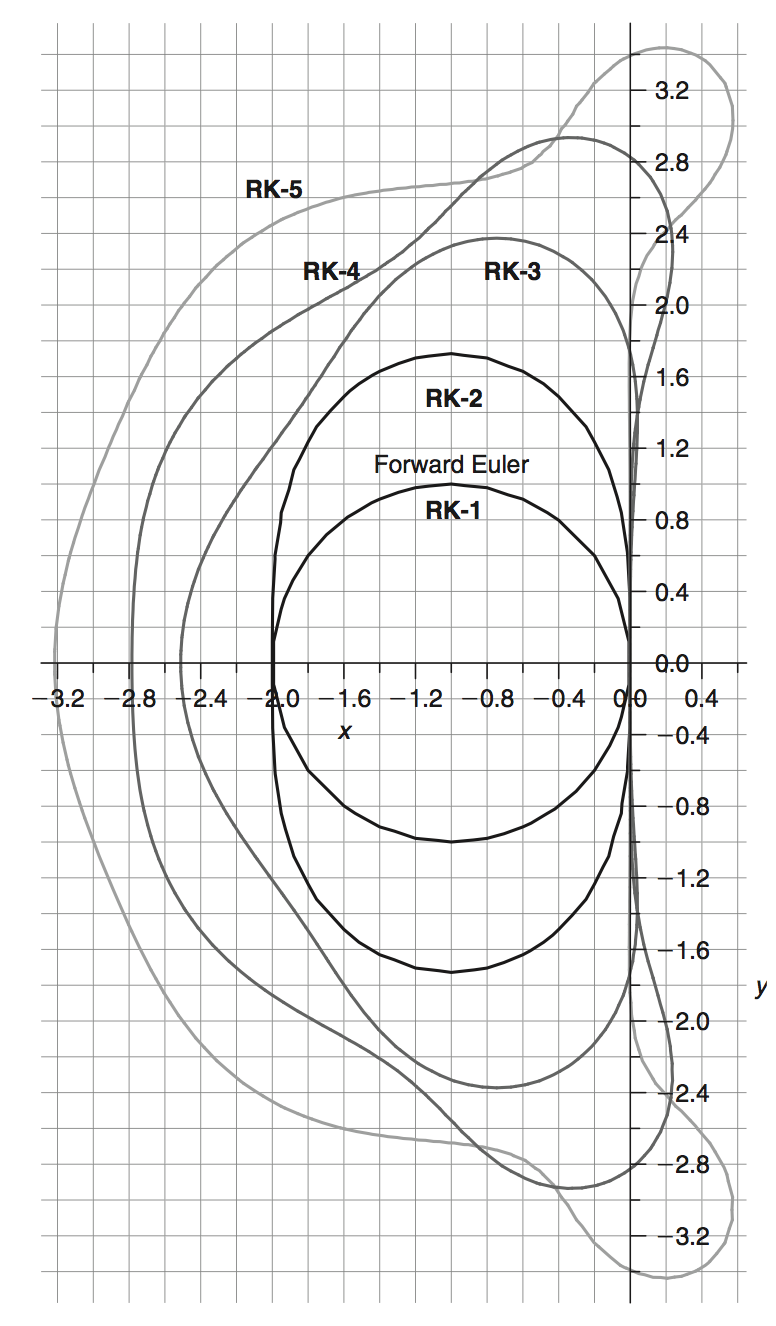
\includegraphics{media/RK-A-stability-regions.png}
    \caption{Región de estabilidad de los métodos de Runge-Kutta}
\end{figure}

%TODO Esto habrá que ponerlo más tarde:
% figureas para los métodos adams, adams-implícitos y adams-bashforth (PECE)

% Iserles pág 60
\begin{theorem}
    Ningún método explícito de Runge-Kutta puede ser $A$-estable.
\end{theorem}

\begin{remark}
    En realidad no hemos definido lo que es
    un método explícito de Runge-Kutta todavía.
    La definición que hemos dado de método de Runge-Kutta
    se corresponde con los métodos explícitos.
    A continuación estudiaremos los métodos implícitos.
\end{remark}

% Iserles pág 67
\begin{theorem}
    El mayor orden de un método multipaso $A$-estable es $2$.
\end{theorem}

A continuación introduciremos

\section{Métodos Implícitos}

Los métodos implícitos son aquellos que
necesitan resolver una ecuación en la que la incógnita
es el siguiente punto de una solución.

\subsection{Método de Euler implícito o hacia atrás}

\begin{method}{Método de Euler hacia atrás}
    El \emph{método de Euler hacia atrás} determina,
    dado el problema \ref{eqn:pvi} y un paso $h > 0$:
%
    \begin{equation}\label{eqn:backwardseulersol}
    \begin{cases}
        w_0 = y_0 \\
        w_{i+1} = w_i + h\cdot f(t_{i+1}, w_{i+1}), \forall i=0,\dots, n-1
    \end{cases}
    \end{equation}
%
    Siendo $t_i = t_0 + i\cdot h$ para $i \in \qty{0,\ldots, n}$.
\end{method}

%TODO el método de euler es estable

\begin{proposition}
    El método de Euler hacia atrás es consistente.

\begin{proof}
    A partir de \eqref{eqn:backwardseulersol}, tenemos que 
    \begin{equation*}
        y(t + h) - y(t) - hf(t+h, y(t+h)) =
        hy'(t + h) + \frac{h^2}{2}y''(\xi) - hy'(t+h) =
        \frac{h^2}{2}y''(\xi).
    \end{equation*}
    Y por tanto, si $\norm{y''}$ está acotada (en el intervalo de resolución),
    $\lim_{h \to 0} \frac{Z(h)}{h} = 0$.
\end{proof}
\end{proposition}

% \begin{remark}
%     Como el método es consistente es también convergente
% \end{remark}

\begin{proposition}
    El método de Euler hacia atrás es $A$-estable.

\begin{proof}
    Fijado el problema $y' = y$, escribimos
    \begin{equation*}
        w_{i+1} = w_i + hf(t_{i+1}, w_{i+1}) = w_i + h\lambda w_{i+1}.
    \end{equation*}
    Reescribiendolo en forma de euación de recurrencia
    llegaríamos a estudiar el polinomio
    \begin{equation*}
        (1 - h\lambda)z - 1 = 0,
    \end{equation*}
    cuya única raíz es $z = \frac{1}{1 - (h\lambda)}$.
    Como
    \begin{equation*}
        \norm{\frac{1}{1 - (h\lambda)}} < 1 \iff
        \norm{1 - (h\lambda)} > 1,
    \end{equation*}
    la región de estabilidad son todos los puntos $(h\lambda) \in \C$
    a distancia mayor que $1$ de $1 \in \C$,
    lo cual incluye todo el semiplano izquierdo.
\end{proof}
\end{proposition}

\subsection{Método del trapecio}

\begin{method}{Método del Trapecio}
    El \emph{método del trapecio} determina,
    dado el problema \ref{eqn:pvi} y un paso $h > 0$:
%
    \begin{equation}\label{eqn:trapezoidalsol}
    \begin{cases}
        w_0 = y_0 \\
        w_{i+1} = w_i + \frac{h}{2}\qty(
            f(t_i, w_i) + f(t_{i+1}, w_{i+1})
        ), \forall i=0,\dots, n-1
    \end{cases}
    \end{equation}
%
    Siendo $t_i = t_0 + i\cdot h$ para $i \in \qty{0,\ldots, n}$.
\end{method}

\begin{proposition}
    El método del trapecio hacia atrás es un método consistente de orden $2$.

\begin{proof}
    A partir de \eqref{eqn:trapezoidalsol}, tenemos que 
    \begin{multline*}
        y(t+h) - y(t) - \frac{h}{2}\qty\bigg(f(t, y(t)) + f(t+h, y(t+h))) = \\
        hy'(t) + \frac{h^2}{2}y''(t) + \frac{h^3}{6}y'''(\xi)
        - \frac{h}{2}\qty\bigg(y'(t) - y'(t+h)) = \\
        hy'(t) + \frac{h^2}{2}y''(t) + \frac{h^3}{6}y'''(\xi)
        - \frac{h}{2}\qty\bigg(2y'(t) + hy''(t) + \frac{h^2}{2}y'''(\xi_2)) = \\
        \frac{h^3}{6}\qty\bigg(y'''(\xi_1) - y'''(\xi_2)).
    \end{multline*}
    Y por tanto, si $\norm{y'''}$ está acotada (en el intervalo de resolución),
    $\norm{\frac{Z(h)}{h}} \le ch^2\max{\norm{y'''}}$
    para una constante $c$,
    y el método es consistente y de orden $2$.
\end{proof}
\end{proposition}

\begin{proposition}
    El método del trapecio es $A$-estable.

\begin{proof}
    Tomando los coeficientes de la ecuación del método,
    \begin{equation*}
        w_{i+1} = w_i + \frac{1}{2}hf(t_i, w_i) + \frac{1}{2}f(t_{i+1}, w_{i+1}),
    \end{equation*}
    obtenemos el polinomio
    $Q(z, h\lambda) = \qty(1 - \frac{h\lambda}{2})z - \qty(1 + \frac{h\lambda}{2})$
    cuya única raíz es
    \begin{equation*}
        z = \frac{1 + \frac{h\lambda}{2}}{1 - \frac{h\lambda}{2}} =
        \frac{2 + h\lambda}{2 - h\lambda}.
    \end{equation*}

    Si tomamos $h\lambda = a + b\iunit$ con $a \le 0$, entonces
    \begin{equation*}
        \norm{\frac{2 + h\lambda}{2 - h\lambda}} =
        \frac{\norm{(2+a) + b\iunit}}{\norm{(2-a) + b\iunit}}
    \end{equation*}
    que es menor que $1$ porque $2 - a > 2 + a$.
    Por tanto, el método es $A$-estable.
\end{proof}
\end{proposition}


\section{Métodos multipaso}

Hasta ahora, al implementar un método de resolución numérica sólo usábamos
$w_i$ para calcular los $w_{i+1}$ \eqref{eqn:diffmet}
ignorando los valores obtenidos anteriormente.
A pesar de que esto parezca obvio pues un p.v.i \eqref{eqn:pvi}
depende únicamente (si $f$ es Lipschitziana) de la condición inicial dada.
Sin embargo, esto solo es cierto si buscamos la solución real del problema,
cuando buscamos una solución computacional
los valores pasados pueden ser de utilidad.
Estos métodos multipaso se construyen, una vez obtenidos los primeros $m$ pasos,
utilizando los $m$ valores anteriores para calcular el valor $w_{i+1}$.
\begin{equation*}
    w_{i+1} = a_0w_{i-m+1} + a_1w_{i-m+2} + \dots + a_{m-1}w_i
        + h_iF(t_i,w_{i-m+1},w{i-m+2},\dots,w_i).
\end{equation*}
Nótese que si ahora tuvieramos $m = 1$,
tendríamos un método a un paso como hasta ahora.
Además ahora tenemos dos tipos de métodos multipaso, pues si usamos $w_{i+1}$
será um método implícito mientras que si no lo usamos será explicito.
Dos ejemplos de estos métodos son
el método explícito de Adams-Bashforth de $4$ pasos
y el método implícito de Adams-Moulton de $3$ pasos.

\begin{method}{Método explícito de Adams-Bashforth de orden $4$}
    El \emph{método de Adams-Bashforth} de orden $4$
    es un método a $4$-pasos.
    \begin{equation}\label{eqn:AB4steps}
        w_{i+1} = w_i + \frac{h}{24}\qty\bigg[
            55f(t_i, w_i) - 59f(t_{i-1}, w_{i-1})
            + 37f(t_{i-2}, w_{i-2}) - 9f(t_{i-3}, w_{i-3})
        ].
    \end{equation}
\end{method}

\begin{proposition}
    El método de Adams-Bashforth de orden $4$
    tiene un error local de truncamiento
    de orden $T_{i+1}(h) = \frac{251}{720}y^5(\xi)h^4$.
\end{proposition}

\begin{method}{Método implícito de Adams-Moulton de orden $4$}
    El \emph{método de Adams-Moulton} de orden $4$
    es un método a $3$-pasos.
    \begin{equation}\label{eqn:AM3steps}
        w_{i+1} = w_i + \frac{h}{24}\qty\bigg[
            9f(t_{i+1}, w_{i+1}) + 19f(t_i, w_i)
            - 5f(t_{i-1}, w_{i-1}) + f(t_{i-2}, w_{i-2})
        ].
    \end{equation}
\end{method}

\begin{proposition}
    El método de Adams-Bashforth de orden $4$
    tiene un error local de truncamiento
    de orden $T_{i+1}(h) = \frac{19}{720}y^5(\xi)h^4$.
\end{proposition}

Podemos ver que ambos métodos requieren de una única evaluación de $f$
en cada paso y que A-M \ref{eqn:AM3steps} tiene un menor e.l.t pero a cambio
requiere alguna forma de despejar $w_{i+1}$.

\begin{remark}
    Estos métodos de Adams se obtienen de lo siguiente
    \begin{equation*}
        y'(t) = f(t,y(t)) \implies
        y(t_{n+1}) - y(t_n) =
        \int\limits_{t_n}^{t_{n+1}} y'(t)dt =
        \int\limits_{t_n}^{t_{n+1}} f(t,y(t)) \dd t
    \end{equation*}
    Si ahora aproximamos $f(t,y(t))$ usando un polinomio interpolador $P(t)$
    en los puntos $t_{i-m+1},\dots,t_i$, tenemos
    \begin{equation*}
        y(t_{n+1}) \approx y(t_n) + \int\limits_{t_n}^{t_{n+1}} P(t)dt
    \end{equation*}
    Por otra parte, los métodos implícitos usan el nodo $(t_{i+1}w_{i+1})$
    a la hora de aproximar la integral.
\end{remark}

En general, los métodos multipaso son de la forma
\begin{equation*}
    w_{i+1} = a_0w_{i-m+1} + \dots + a_{m-1}w_i + h[
        b_0f(t_{i+1-m},w_{i+1-m}) + \dots + b_{m-1}f(t_i,w_i)
        + b_mf(t_{i+1},w_{i+1})
    ],
\end{equation*}
donde los $m$ primeros $w_j$ han sido calculados con otro método de un paso.
Si $b_m = 0$ entonces el método es explícito, en otro caso es implícito.
Resolver la ecuación implicita para $w_{i+1}$ no se puede hacer, en general,
de forma analítica.

\section{Teoría general de Convergencia}

Con los métodos multipaso hay que tener cuidado pues usamos
sucesiones recurrentes de orden mayor que uno,
lo que nos puede dar problemas por estar mal condicionada
(a parte de los problemas generados por el propio método).
Por ello introducimos las siguientes definiciones:

\begin{definition}
    Un método se dice \emph{consistente} (o \emph{compatible})
    con el p.v.i. que aproxima si
    \begin{equation*}
        \lim\nolimits_{h\to 0} \max{\norm{T_{i+1}(h)}} = 0.
	\end{equation*}
	El método se dice de orden $p$, $p \geq 1$, si $p$ es el mayor entero
	tal que $\max{\norm*{T_{i+1}(h)}} = \theta(h^p)$.
\end{definition}

Naturalmente solo consideraremos los métodos consistentes y de orden tan
alto como podamos encontrar teniendo un coste razonable.

\begin{definition}
    %TODO método en diferencias es multipaso o qué?
    % Hay un lío de términos importante
    Un método en diferencias
    \begin{equation*}
        w_{i+1} = \sum_{j=1}^m {a_{j-1}w_{i-m+j}}
            + hF(t_i,w_{i-m+1}, \dots, w_i,w_{i+1},h)
    \end{equation*}
    se dice convergente si
    \begin{equation*}
        \lim\nolimits_{h \to 0} \max{\norm{Y(t_i)-w_i}} = 0.
    \end{equation*}
\end{definition}

Un método convergente nos resuelve el problema en caso de una
implementacion de ``aritmética infinita''.
Lamentablemente solo disponemos de ordenadores de aritmética finita,
luego nuestros métodos no son los deseados sino los aproximados. %TODO EIN?
Por eso, introducimos la noción de método estable.

\begin{definition}
    Un método en diferencias se dice estable
    si al generar una segunda solución aproximada de la forma
    \begin{equation*}
        \tw_{i+1} = \sum_{j=1}^m {a_{j-1}\tw_{i-m+j}}
            + h F(t_i,\tw_{i-m+j}, \dots, \tw_i,\tw_{i+1},h) + \epsilon'_i,
    \end{equation*}
    existe una constante $M$, independiente de $h$, tal que
    \begin{equation*} \label{stab}
        \max_{m \leq n \leq N}{\norm{\tw_n - w_n}} \leq M\qty[
            \max_{0 \leq i \le m-1}{\norm{\tw_i - w_i}}
            + \sum_{m \leq j \leq N} \norm{\epsilon'_j}
        ]
    \end{equation*}
\end{definition}

\begin{remark}
    %TODO una referencia estaría increible en vd
    Esto no contradice el resultado que obtuvimos para Euler, pues
    %TODO esto pq?
    $\sum\norm{\epsilon_j} \approx n\epsilon \approx \frac{b-a}{h}\epsilon$.
\end{remark}

\begin{theorem}
    Si un método en diferencias
    \begin{equation*}
        w_{i+1} = \sum_{j=1}^m {a_{j-1}w_{i-m+j}}
            + hF(t_i,w_{i-m+j}, \dots, w_i,w_{i+1},h)
    \end{equation*}
    es estable y consistente, entonces es convergente.
    Si, además, es de orden $p \geq 1$, se tiene
    \begin{equation*}
        \max_{0 \leq n \leq N}\norm{x(t_n) - w_n} \leq M\qty\bigg[
            \max_{0 \leq i \leq m-1} \norm{x(t_i) - w_i} + Kh
            ]
    \end{equation*}
    Para constantes adecuadas M y K.
\end{theorem}

\begin{proof}
    Sea $\epsilon_i = hT_i(h_i)$ y utilicemos la estabilidad
    con $\tilde{w}_n = Y(t_n)$. Se tiene que
    \begin{equation*}
        \max_{0 \leq n \leq N}\norm{Y(t_n) - w_n} \leq M\qty\bigg[
            \max_{0 \leq i \leq m-1}\norm{Y(t_i) - w_i}
            + \sum_{m-1\leq n \leq N}\norm{\epsilon_n}
        ]
    \end{equation*}
    para algún $m$. Pero
    \begin{equation*}
        \sum_{m \leq n \leq N} \norm{\epsilon_n} =
        \sum_{m \leq n \leq N} h\norm{T_{n+1}(h)} \leq
        \qty(\sum_{m \leq n \leq N} h)
            \max_{m \leq n \leq N}\norm{T_{n+1}(h)} \leq
        (b-a)\max_{m \leq n \leq N}\norm{T_{n+1}(h)},
    \end{equation*}
    donde esta última tiende a $0$ cunado $h$ tiende a $0$
    por la condición de consistencia.
    Si además $\max\norm{T_{n+1}(h)} = O(h^p)$,
    $\max\norm{T_i+1I(h)} \leq \frac{kh^p}{b-a}$ para algún $K$
    de ahí el resultado.
\end{proof}

%TODO este teorema está fatal hay que mirarlo en el burden
\begin{theorem}
    Sea $w_{i+1} = w_i + h\phi(t, w_i, h)$ un método a un paso tal que
    $\phi(t_i, w_i, h)$ es continua y lipschitziana en $w_i$.
    Entonces existe $h_0 > 0$ tal que para todo $h < h_0$,
    \begin{enumerate}
        \item El método es estable
        \item El método es convergente si es consistente,
        lo que ocurre si $\phi(t, y, 0) = f(t, y)$ para todo $t$.
    \end{enumerate}
\end{theorem}

\begin{proof}
    Sea $L$ la constante de lipschitz de $\phi$ y
    sean $w_{i+1} = w_i + h\phi(t, w_i, h)$ y
    $\tw_{i+1} = h\phi(t, \tw_i, h) + \epsilon_i$.
    Entonces
    \begin{align*}
        \norm{\tw_{i+1} - w_{i+1}} & {} \le
            (1 + hL)\norm{\tw_i - w_i} + \norm{\epsilon_i} \\
        & \le (1 + hL)^2\norm{\tw_{i-1} - w_{i-1}}
            + (1 + hL)\norm{\epsilon_{i-1}} + \norm{\epsilon_i} \le \ldots \\
        \ldots & \le (1 + hL)^{i+1}\norm{\tw_0 - w_0} + \qty[
            \norm{\epsilon_i} + (1 + hL)\norm{\epsilon_{i-1}} + \dots
            + (1 + hL)^i\norm{\epsilon_0}
        ] \\
        & \le (1 + hL)^i\qty(
            \norm{\tw_0 - w_0} + \sum_{j=0}^i \norm{\epsilon_j}
        ).
    \end{align*}
    Lo que demuestra que el método es estable.

    Estudiamos ahora el error de truncamiento.
    \begin{multline*}
        Z_i(h) = \frac{y(t_i + h) - y(t)}{h} - \phi(t, y(t_i), h) =
        y'(\xi_i) - \phi(t, y(t_i), h) = \\
        f(\xi_i, y(\xi_i)) - \phi(t, y(t_i), h) =
        f(\xi_i, y(\xi_i)) - \phi(\xi_i, y(\xi_i), 0)
            + \phi(\xi_i, y(\xi_i), 0) - \phi(t, y(t_i), h).
    \end{multline*}
    Por la continuidad uniforme de la función
    $(t, h) \mapsto \phi(t, y(t), h)$
    sobre $[a, b] \times [0, h_0]$,
    dado $\epsilon > 0$ existe $h_0 > 0$ tal que si $h < h_0$,
    entonces como $\abs{\delta_i - t_i} < h$,
    \begin{equation*}
        \norm{\phi(\xi_i, y(\xi_i), 0) - \phi(t, y(t_i), h)} < \epsilon.
    \end{equation*}
    Por tanto, $\lim_{h \to 0} Z_i(h) = 0$
    si $f(t_i, y(t_i)) = \phi(t_i, y(t_i), 0)$.
\end{proof}

\subsection{Estudio de la estabilidad para métodos multipaso}

Estudiar la estabilidad de los métodos a $m$ pasos es más complicado.
En realidad, para estudiar la estabilidad basta hacerlo con el problema
$y' = 0$, $y(0) = \alpha$,
pero la demostración de este hecho no forma parte de estos apuntes.

Dado un método multipaso estándar a $m$ pasos,
\begin{equation*}
    w_i = a_0w_{i-m} + \dots + a_{m-1}w_{m-1} + h\qty\bigg[
        b_0f(t_{i-m}, w_{i-m}) + \dots + b_{m-1}f(t_{i-1}, w_{i-1})
        + b_mf(t_i, w_i)
    ]
\end{equation*}
el siguiente punto para el problema de prueba con $y' = 0$ se calcularía
siguiendo la ecuación de recurrencia
\begin{equation*}
    w_i = a_0w_{i-m} + \dots + a_{m-1}w_{m-1} + a_mw_m,
\end{equation*}
cuyo polinomio característico tiene raíces que satisfacen
\begin{equation*}
    z^m = a_0 + \dots + a_{m-1}z^{m-1}.
\end{equation*}
Si todas las raíces reales, $\lambda_1,\dots,\lambda_n$, fuesen distintas,
la ecuación general sería
\begin{equation*}
    w_n = \sum_{j=1}^m c_j\lambda_j^n
\end{equation*}
con los $c_j$ en función de $m$ puntos iniciales.

Lo primero que podemos afirmar es que como $y(t) = \alpha$ es una solución,
si el método tiene error local de truncamiento $\theta(h^p)$, $p \ge 1$,
$w_n = \alpha$ debe ser una posible solución:
\begin{equation*}
    \alpha = a_0 + a_1\alpha + \dots + a_{m-1}\alpha.
\end{equation*}
Es decir, $\lambda = 1$ es una de las raíces del polinomio caracerístico.
por lo que las soluciones son de la forma
\begin{equation*}
    w_n = c_1\alpha + \sum_{j=2}^m c_j\lambda_j^n,
\end{equation*}
y para nuestra ecuación de prueba sería $c_j = 0$ para todo $j$.

Para estudiar la estabilidad,
nos interesa que acotando los errores de redondeo en las condiciones iniciales
se acoten también los errores en la solución calculada.
Eso motiva la siguiente definición.

\begin{definition}
    Sean $\lambda_1,\ldots,\lambda_n$ las $n$ raíces del
    polinomio característico
    \begin{equation*}
        \lambda^m - a_{m-1}z^{m-1} - a_{m-2}z^{m-2} - \dots - a_0
    \end{equation*}
    de un método a $m$ pasos
    \begin{equation}\label{eqn:multistep}
        w_{i+1} = a_0w_{i-m+1} + a_1w{i-m+2} + \dots + a_{m-1}w_i
            + h_iF(t_i,w_{i-m+1},w{i-m+2},\dots,w_i).
    \end{equation}
    El método cumple la \emph{condición de raíz} si
    $\abs{\lambda_i} \le 1$ para todo $i = 1,\ldots, m$
    %TODO este tipo de añadidos que son necesarios si no asumimos todas distintas
    % hay que ver si los quitamos porque con Esquembre no lo hemos visto
    % pero especificamos que lo hemos quitado
    % o si lo dejamos y lo marcamos con otro color por ejemplo
    % o si lo quitamos
    y todas las raíces de valor absoluto uno son simples.
\end{definition}

\begin{theorem}
    Un método multipaso es estable si y solo si cumple la condición de raíz.
    Además, si el método es consistente,
    que sea estable es equivalente a que sea convergente.
\end{theorem}

\section{Implementación de los métodos de Adams. Predictor-corrector}

Estos métodos sirven para obtener lo mejor de los métodos explícito e implícito,
la completitud del primero y el mejor error del segundo,y se consiguen usando
el implícito para corregir la predicción del método explícito. Por ejemplo,
uno de estos métodos  sería usar como predictor el método de Adams-Bashforth 
de $4$ pasos (\cref{eqn:AB4steps}) y como corrector el método de Adams-Moulton
de $3$ pasos (\cref{eqn:AM3steps}).

De manera parecida a RKF, %TODO referencia a RKF
el método predictor-corrector obtiene, cada vez,
dos aproximaciones de la solución,
una obtenida de uno del predictor y otra del corrector.
Por la definición de error local de truncamiento tenemos que
\begin{gather*}
    y(t_{i+1}) = y(t_i) + \frac{h}{24}[
        55f(t_i,y(t_i) - 59f(t_{i-1},y(t_{i-1})) + 37f(t_{i-2}, y(t_{i-2}))
        - 9f(t_{w-3},y(t_{i-3})))
    ] + \frac{251}{720}y^{(5)}(\xi)h^5  \\
    y(t_{i+1}) = y(t_i) + \frac{h}{24}[
        9f(t_{w+1},y(t_{i+1})) + 19f(t_i,y(t_i) - 5f(t_{i-1},y(t_{i-1}))
        + f(t_{i-2}, y(t_{i-2})))
    ] - \frac{19}{720}y^{(5)}(\mu)h^5
\end{gather*}
Y si ahora identificamos los $w_j \approx y(t_j)$ para $j = 0,1,\dots, i$,
tenemos que
\begin{equation*} 
    y(t_{i+1} - w_{i+1}^{(0)}) \approx {} 
        \frac{251}{720}y^{(5)}(\xi)h^5
\end{equation*}
\begin{equation} \label{eqn:pred-corr}
    y(t_{i+1} - w_{i+1}^{(1)}) \approx {} 
        \frac{-19}{720}y^{(5)}(\mu)h^5.
\end{equation}
Si además, $h$ es suficientemente pequeño entonces
$y^{(5)}(\xi) \approx y^{(5)}(\mu)$
y restando
\begin{align*}
    w_{i+1}^{(1)} - w_{i+1}^{(0)} \approx 
        \frac{h^6}{720}\qty[251y^{(5)}(\xi) + 19y^{(5)}(\mu)] \approx &
        \frac{27}{72}h^5y^{(5)}(\mu) = \frac{3}{8}h^5y^(\mu) \\
    y^{(5)}(\mu) = \frac{8}{3h^5}(w_{i+1}^{(1)} - w_{i+1}^{(0)}) &
\end{align*}
Por lo tanto, de \ref{eqn:pred-corr} tenemos
\begin{equation*}
    y(t_{i+1}) - w_{i+1}^{(1)} \approx \frac{-19 * 8}{720 * 3}(w_{i+1}^{(1)} - w_{i+1}^{(0)})
\end{equation*}
Es decir
\begin{equation*}
    \tilde{e}_r(h) = \frac{19}{270}\norm{w_{i+1}^{(0)} - w_{i+1}^{(1)}}   
\end{equation*}
es una aproximación del error para un método de orden 4.
Luego dada una tolerancia $\epsilon > 0$, usando la estimación
local del paso del hijo de Ricardo tenemos
\begin{equation*}
    q = \bigg(\frac{\epsilon h}{\tilde{e}_r(h)}\bigg)^{1/4} \approx 
        2.48\bigg(\frac{\epsilon h}{\norm{w_{i+1}^{(0)} - w_{i+1}^{(1)}}}\bigg)^{1/4}
\end{equation*}
%TODO dice algo de ser mas consevador que blablabla
Por otra parte, cambiar el paso supone reiniciar los
$4$ primeros pasos de modo que se ignora el cambio de paso 
si tenemos que 
\begin{equation*}
    \frac{\epsilon h}{10} < \tilde{e}(h)
\end{equation*}

\input{src/4}


\end{document}
